\documentclass[12pt]{beamer}
\usepackage{mathtools}
\useoutertheme{infolines}
\usetheme{default}
\usefonttheme{serif}
%\usefonttheme{structuresmallcapsserif}
\hypersetup{colorlinks=true,linkcolor=blue}
\setbeamertemplate{navigation symbols}{}
\author{Mittereder, \textit{et. al.}}
\definecolor{darkgreen}{rgb}{0,.5,0}
\setlength{\parskip}{.1in}

\begin{document}

\begin{frame}[c]{} % Justin

\begin{center}
\Large
Exploring the Impact of Social Network Density\\and Agent Openness on Societal Polarization

\footnotesize
\vspace{.3in}
CSS 2021 --- Santa Fe, New Mexico (sorta)\\
\vspace{.1in}
Justin Mittereder, Robert S.~W.~Carroll, Brandon Frulla, Stephen Davies\\
\scriptsize
\smallskip
Dept of Computer Science\\
University of Mary Washington\\
Fredericksburg, Virginia, USA\\
\end{center}

\end{frame}

\begin{frame}[c]{Defining polarization} % Stephen

\large

\centering
``America is becoming increasingly polarized..."

% TODO: get JAn 6th photo
\vspace{-.2in}
\begin{figure}
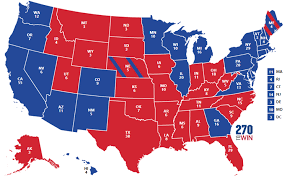
\includegraphics[width=0.35\textwidth]{usa.png}
\end{figure}
\pause
\vspace{-.2in}
What does this actually mean?
\vspace{-.15in}
\pause

\small
\begin{itemize}
\itemsep.1em
\item People's views becoming more \textit{extreme}?
\pause
\item People becoming more \textit{stubborn}? (less willing to reconsider views)
\pause
\item People only associating with like-minded others?
\end{itemize}

\end{frame}

\begin{frame}[c]{Proxy \#1: Assortativity coefficient} % Justin

% TODO: add slides from extravaganza, and explain assortativity well

% explain why we think this is a measure of polarization

% "echo chambers"

\end{frame}


\begin{frame}[c]{Proxy \#2: Issue Alignment} % Stephen

We define \textbf{Issue Alignment} (IA) as the tendency for people who agree on
one issue to also agree on other (unrelated) issues.

{\tiny \color{red} 
Stephen TODO:

\begin{itemize}
\itemsep.1em
\item Illustrative list of typical left vs. right positions
\item Ask: in your experience, does this hold true?
\end{itemize}
}

\end{frame}

\begin{frame}[c]{The model}  % Justin

% Describe in selected detail the model

% N heterogeneous agents who encounter each other on a social network.

% ER edge prob is a parameter

% Multiple continuous opinions 

\end{frame}


\begin{frame}[c]{Traditional BC}  % Justin

% Here is traditional bounded confidence (BC) from Hegelsmen-Krause

% Show one number line and two peeps

\end{frame}


\begin{frame}[c]{CI2 - attraction only}  % Justin

We define \textbf{Cross-Issue Influence} (CI2) as the effect that a person's
social contact can have on one of their opinions based on their agreement (or
disagreement) on a different issue.

% Show two number line and two peeps, with an attraction due to openness

\end{frame}


\begin{frame}[c]{CI2 - add repulsion}  % Justin

% Show two number line and two peeps, with a repulsion due to disgust

% Also show the Justin threshold diagram with red & green regions

% And cite Griffin, Em (2011). A First Look at Communication Theory. New York,
% New York: McGraw Hill. pp. 194–204.

\end{frame}

\begin{frame}[c]{Fig 1 explained}  % Justin

Fewer (meaningful) social connections = higher polarization BUT only at the low
end.

\end{frame}

\begin{frame}[c]{Fig 2 explained}  % Justin

%TODO: Justin verify
%(Just for completeness, rerun paper graph Figure 2 with a much lower value of
%edge prob (how about .05 instead of .5, for instance.) Then we’ll verify the
%null hypothesis that “openness does not impact assortativity.”)

openness threshold surprisingly does not seem to impact assortativity.

\end{frame}

\begin{frame}[c]{Proxy \#2: Issue Alignment} % Stephen

Reminder: define \textbf{Issue Alignment} (IA) as the tendency for people who agree on
one issue to also agree on other (unrelated) issues.

{\tiny \color{red} 
Stephen TODO:

\begin{itemize}
\itemsep.1em
\item Illustrative list of typical left vs. right positions
\item Ask: in your experience, does this hold true?
\end{itemize}
}

\end{frame}
\begin{frame}[c]{One possible explanation for IA} % Stephen

{\tiny \color{red} 
Stephen TODO:

Perhaps there is some deep underlying principle to people's ideologies that
connects seemingly unconnected issues. (Maybe for some deep reason it actually
makes sense that people who are pro-life are also pro-gun, and anti-tax, and
anti-vacc.)
}

\end{frame}

\begin{frame}[c]{Another possible explanation for IA} % Stephen

{\tiny \color{red} 
Stephen TODO:

Perhaps a small number of popular media outlets each articulates a number of
opinions on various issues. The people who listen to them are naturally
influenced to each of these different opinion values, and thus become ``issue
aligned."
}

\end{frame}

\begin{frame}[c]{A third possible explanation for IA} % Stephen

CI2!

{\tiny \color{red} 
Stephen TODO:

We wish there was more justification in the social psych lit for this, but we
have to fall back on (1) homophily and (2) common sense.
}

{\small \color{red} 
Big idea: even without any underlying ideological connection between issues,
and even without media influence, IA will naturally develop solely due to CI2.
In other words, CI2 is sufficient for IA. (Wide reaching implications on how we
interpret the causes of the polarization phenomenon, and what societal changes
might be necessary to reduce it.)
}

\end{frame}

\begin{frame}[c]{IA example} % Stephen

\end{frame}


\begin{frame}[c]{Define "buckets"} % Stephen

\end{frame}


\begin{frame}[c]{Define "clone pair" / anti-clone pair} % Stephen

\end{frame}



\begin{frame}[c]{Census plot w/o CI2} % Stephen

\end{frame}

\begin{frame}[c]{Census plot w/ CI2} % Stephen

\end{frame}

\begin{frame}[c]{Heat maps: showing interplay of openness and disgust threshold
with and without CI2} % Stephen

\end{frame}


% Tuck-away slide
%\begin{frame}[c]{Diametricity}
%
%One other way to define polarization is extremity of views.
%
%Fact: if CI2 is employed, the model always (?) produces exactly two buckets,
%and all the opinions in those buckets are at the poles.
%
%Fact: if only I2 is employed, there will normally be many buckets (often one
%for each combination of fully-polarized opinions; i.e., a (0,0,0) bucket, a
%(0,0,1), (0,0,2), (0,1,0), ...)
%
%\end{frame}

\begin{frame}[c]{Discussion and takeaways}  % Stephen & Justin

\end{frame}

\begin{frame}[c]{}

\begin{center}
\Large
Exploring the Impact of Social Network Density\\and Agent Openness on Societal Polarization

\footnotesize
\vspace{.3in}
CSS 2021 --- Santa Fe, New Mexico (sorta)\\
\vspace{.1in}
Justin Mittereder, Robert S.~W.~Carroll, Brandon Frulla, Stephen Davies\\
\smallskip
\scriptsize
Dept of Computer Science\\
University of Mary Washington\\
Fredericksburg, Virginia, USA\\
\end{center}

\end{frame}
\end{document}
